% What is the current state of the system
\chapter{Current systems for safe navigation}
\label{app:systems}
Before developing new systems and procedures to improve safety, the first step is to know what is currently available. Thereby should be considered how different types of information can be supplied. Nowadays decisions on navigation are taken from the bridge. Thus all information must be available there. In this chapter these elements will first be discussed, how they are in theory. This is followed by a discussion on the differences between this theory and practice. Which results in a conclusion on relevant systems for the communication between manned and unmanned ships.

\section{Bridge system elements}
To gain insight in a structured way, the bridge is split into four elements as described by DNV-GL. The human operator, procedures, technical system and the human-machine interface \cite{DNVGL2011}, as shown in figure \ref{fig:Bridge-system-elements}. This section describes every element in more detail.

\begin{figure}[H]
	\centering
	\includegraphics[width=0.72\textwidth]{Bridge-system-elements.png}
	\caption{Bridge system elements}
	\label{fig:Bridge-system-elements}
\end{figure}

\subsection{Technical system}
The first element which will be discussed are the instruments and equipment at the bridge, the technical system. The different classification societies prescribe the equipment which is obligated to have at the bridge. These are based on the regulations for navigational equipment on board of ships from the \ac{SOLAS}, a modern ship should at least have:
\begin{multicols}{2}
	\begin{itemize}
		\item Magnetic compass
		\item Gyro compass
		\item \ac{ECDIS}
		\item Transmitting heading device
		\item \acf{AIS}
		\item Receiver for \ac{GNSS}
		\item Internal communication system
		\item \ac{BNWAS}
		\item Telephone for external communication
		\item Radar
		\item Radar beacon
		\item Daylight signaling lamp
		\item Speed and distance measuring device
		\item Echo sounding device
		\item Rudder, propeller, thrust, pitch and operational mode indicators
		\item Rate of turn indicator
	\end{itemize}
\end{multicols}

Based on this list, DNV-GL demands at least the following equipment shall be installed at the bridge \cite{DNVGL2011}. The equipment may have different roles. To control the ship, to present information, or to communicate:
\begin{multicols}{2}
	\begin{itemize}
		\item Propulsion control
		\item Emergency stop machinery
		\item Manual steering device
		\item Steering mode selector switch
		\item Heading control
		\item Window wiper and wash controls
		\item Control of dimmers for indicators and displays
		\item Steering gear pumps
		\item Gyrocompass selector switch
		\item Navtex receiver
		\item \acf{ARPA}
		\item \acf{ECDIS}
		\item \acf{AIS} transceiver
		\item General alarm control
		\item \acf{VHF} unit
		\item Whistle and manoeuvring light push buttons
		\item Internal communication equipment
		\item Central alert management system
	\end{itemize}
\end{multicols}

Some of these systems will be highlighted to show the relevance for the development of unmanned vessels, as these systems are currently the most important systems while navigating. Thereby should be considered that more details on underlying procedures are given later in this chapter. 

\subsubsection{\acf{Navtex}}
Navtex (Navigational Telex) is an international automated medium frequency direct-printing service for delivery of navigational and meteorological warnings and forecasts, as well as urgent maritime safety information to ships. Navtex was developed to provide a low-cost, simple, and automated means of receiving this information aboard ships at sea within approximately 370 km (200 nautical miles) off shore.
Transmissions are typically transmitted from the National Weather Authority, Coast Guard or other navigational authority.
The system is an important element in the Global Maritime Distress Safety System (GMDSS). Therefore does \ac{SOLAS} mandate certain classes of vessels must carry Navtex.
Examples of messages which can be received are:
\begin{multicols}{2}
	\begin{itemize}
		\item Navigational warnings
		\item Meteorological warnings
		\item Meteorological forecasts
		\item Search \& rescue information
		\item Piracy information
		\item \ac{AIS} messages
	\end{itemize}
\end{multicols}
The receiver automatically prints the messages. The officer of watch keeps track of the received messages, and anticipates on them when necessary.

\subsubsection{\acf{VHF}}
Marine VHF radio refers to the radio frequency range between 156 and 174 MHz. In the official language of the International Telecommunication Union the band is called the VHF maritime mobile band.
A marine VHF set is a combined transmitter and receiver and only operates on standard, international frequencies known as channels. For example is channel 16 (156.8 MHz) the international calling and distress channel. Transmission power ranges between 1 and 25 watts, giving a maximum range of up to about 60 nautical miles (111 km) between aerials mounted on tall ships and hills, and 5 nautical miles (9 km) between aerials mounted on small boats at sea level (figure \ref{fig:vhf-radio}). Frequency modulation (FM) is used, with vertical polarization, meaning that antennas have to be vertical in order to have good reception.

\begin{figure}[H]
	\centering
	\includegraphics[width=0.9\textwidth]{VHF-radio.png}
	\caption{\acf{VHF}}
	\label{fig:vhf-radio}
\end{figure}

Modern-day marine VHF radios offer not only basic transmit and receive capabilities. Permanently mounted marine VHF radios on seagoing vessels are required to have certification of some level of "Digital Selective Calling" (DSC) capability, to allow a distress signal to be sent with a single button press.

Marine VHF mostly uses "simplex" transmission, where communication can only take place in one direction at a time. A transmit button on the set or microphone determines whether it is operating as a transmitter or a receiver. Some channels, however, are "duplex" transmission channels where communication can take place in both directions simultaneously when the equipment on both ends allow it (full duplex), otherwise "semi-duplex" is used. Each duplex channel has two frequency assignments. Duplex channels can be used to place calls on the public telephone system for a fee via a marine operator. When full duplex is used, the call is similar to one using a mobile phone or landlines. When semi-duplex is used, voice is only carried one way at a time and the party on the boat must press the transmit button only when speaking. This facility is still available in some areas, though its use has largely died out with the advent of mobile and satellite phones. Marine VHF radios can also receive weather radio broadcasts, where they are available.

\subsubsection{\acf{ARPA}}
Radars have been playing a vital role in ship navigation for several decades now, assisting in collision avoidance and early detection of obstacles.The history of marine radars goes a long way back to the time of World War II, when radars were introduced and effectively used by war ships for tracking and detection. Radar technology has improved immensely from post-WWII period to the present and the application of computer technology to commercial marine radar sets resulted in the introduction of Automatic Radar Plotting Aids (ARPA). A print-screen of an ARPA systems can be seen in figure \ref{fig:ARPA}.

\begin{figure}[H]
	\centering
	\includegraphics[width=0.72\textwidth]{ARPA.png}
	\caption{\acf{ARPA}}
	\label{fig:ARPA}
\end{figure}

Automatic radar plotting aids are essentially utilized to improve the standard of collision avoidance at sea. Primarily designed as anti-collision radar, the ARPA technology removed the chore of plotting targets manually on a reflection plotter or separate plotting aid. The system is able to acquire automatically and constantly monitor number of targets, plot their speeds and courses, present these as vectors on the display screen, updated with each sweep of the antenna, and calculate their closest points of approach to own ship and the time before that will occur.

\subsubsection{\acf{ECDIS}}
The \acf{ECDIS} is a development in the navigational chart system used in naval vessels and ships. With the use of the \acf{ENC} system, it has become easier for a ship’s navigating crew to pinpoint locations and attain directions. ECDIS equipment complying with SOLAS requirements can be used as an alternative to paper charts. Besides enhancing navigational safety, ECDIS greatly eases the navigator’s workload with its automatic capabilities such as route planning, route monitoring, automatic ETA computation and ENC updating. In addition, ECDIS provides many other sophisticated navigation and safety features, including continuous data recording for later analysis. How the ECDIS is integrated in the bridge can be seen in figure \ref{fig:ECDIS}.

\begin{figure}[H]
	\centering
	\includegraphics[width=0.72\textwidth]{ECDIS.jpg}
	\caption{\acf{ECDIS}}
	\label{fig:ECDIS}
\end{figure}

The ECDIS utilises the feature of the Global Positioning System (GPS) to successfully pinpoint the navigational points. It also has to be noted that the ECDIS adheres to the stipulations set by the International Maritime Organisation, and thus it adds to the trustworthiness of the electronic chart system. ECDIS is basically a navigational information system, interfaced with other navigational equipments such as the GPS, Gyro, RADAR, ARPA, Echo Sounder etc.

\subsubsection{\acf{AIS}}
\ac{AIS} is designed to be capable of providing information about the ship to other ships and to coastal authorities automatically. The \ac{SOLAS} regulations require \ac{AIS} to be fitted aboard all ships of 300 gross tonnage and upwards engaged on international voyages, cargo ships of 500 gross tonnage and upwards not engaged on international voyages and all passenger ships irrespective of size. The requirement became effective for all ships by 31 December 2004, this means there are still ships which do not have \ac{AIS}. Ships fitted with \ac{AIS} shall maintain \ac{AIS} in operation at all times except where international agreements, rules or standards provide for the protection of navigational information.

The regulations require the \ac{AIS} to provide information on ship's identity, type, position, course, speed, navigational status and other safety-related information. Which will be automatically send to appropriately equipped shore stations, others ships and aircrafts. While also being able to receive such information automatically from similarly fitted ships, to monitor and track them. Lastly they should be able to exchange data with shore-based facilities. 

Originally the messages were send regularly via a \ac{VHF} transmitter. The information originates partly from ship's navigational sensors. Other information, such as the vessel name and \ac{VHF} call sign, is programmed when installing the equipment. Some information must be filled in by hand, such as the status or destination, which is often forgotten. The received information can be displayed on a screen or chart plotter, showing the other vessels' positions in much the same manner as a radar display. Data is transmitted via a tracking system which makes use of a Self-Organized Time Division Multiple Access (SOTDMA).

There are different types of transmitters. Depending on the object it is installed on. This determines what kind of messages can be send and which protocol is used to access \ac{AIS} slots. Below relevant types are described:
\begin{itemize}
	\item Class A, the most common type of \ac{AIS} transceiver for large merchant vessels.
	\item Class B, \ac{AIS} for smaller vessels.
	\item Base station, shored-based \ac{AIS} transceiver, able to maanage \ac{AIS} slots.
	\item Aids to navigation, shore- or buoy based transceiver operating in fixed time-slots. Designed to collect and transmit data related to sea and weather conditions, or forward \ac{AIS} messages to extend reach.
	\item Search and rescue transceiver, designed to function as an emergency distress beacon, with high probability of success for transmission.
\end{itemize}

As mentioned before, there are different types of \ac{AIS} messages, identification numbers are used to identify the type of message within the NMEA string. The following types of messages are relevant for this research and the development of unmanned ships \cite{USCG2018}:
\begin{itemize}
	\item Position report, reports navigational information.
	\item Standard class B equipment position report, less detailed report for vessels using class B transmitters.
	\item Base station report, used by base stations to indicate presence.
	\item Static and voyage related data, gives information on a ship and its trip
	\item Binary addressed message and acknowledgment, an addressed point-to-point message with unspecified binary payload.
	\item Binary broadcast message, broadcast message with unspecified binary payload.
	\item Standard Search and Rescue Aircraft Position Report, used by an aircraft (helicopter or airplane) which is involved with search and rescue operation on the sea (i.e. search for and recovery of survivors of an accident at sea).
	\item Addressed Safety-Related message and response, used to send text messages to a specified vessel.
	\item Interrogation, used by a base station to get the status of up to 2 other AIS devices.
	\item Aids-to-navigation report, used by an (AtN) aid to navigation device (buoys, lighthouse, etc.).
	\item Multiple slot binary message with communications state, used to transmit binary data from one device to another.
\end{itemize}

\subsection{Man/machine interface}
Previously all information was plotted by hand on navigational charts. With the developments of integrated bridge systems and for example the \ac{ECDIS}, this is not necessary. This also means that a digital representation of the environment is already being made. Including calculations, relevant for navigational safety. These also give warnings to avoid collisions or represent information received via \ac{VHF}. This is done in a way which is more easy to interpret by the officer of watch, as for example \ac{AIS}, \ac{ENC} and the radar are combined. Examples of the different systems can be found in figure \ref{fig:ECDIS-example}.

\begin{figure}[p]
	\centering
	
	\begin{subfigure}[b]{0.6\textwidth}
		\includegraphics[width=\textwidth]{ECDIS-Radar.jpg}
		\caption{Separate screens for ECDIS and Radar}
	\end{subfigure}
	\hfill
	\begin{subfigure}[b]{0.37\textwidth}
		\includegraphics[width=\textwidth]{ECDIS-Radar-overlay.png}
		\caption{Radar overlay on ECDIS}
	\end{subfigure}
	
	\caption{Radar and ECDIS}
	\label{fig:ECDIS-example}
	
\end{figure}

These screens are all integrated in some way into the bridge console. Depending on the size of the vessel, the lay-out may differ. Although, there are also regulations for the placement of systems in \ac{SOLAS}. Examples of these bridge layouts can be found in figure \ref{fig:Bridge-system-elements}.

\begin{figure}[p]
	\centering
	
	\begin{subfigure}[b]{0.45\textwidth}
		\includegraphics[width=\textwidth]{brug-alphatron.jpg}
		\caption{Alphatron AlphaBridge}
	\end{subfigure}
	\hfill
	\begin{subfigure}[b]{0.45\textwidth}
		\includegraphics[width=\textwidth]{Brug-ASD-2310-PATRIOT.JPG}
		\caption{DAMEN ASD Tug 2310 (Patriot)}
	\end{subfigure}
	\hfill
	\begin{subfigure}[b]{0.45\textwidth}
		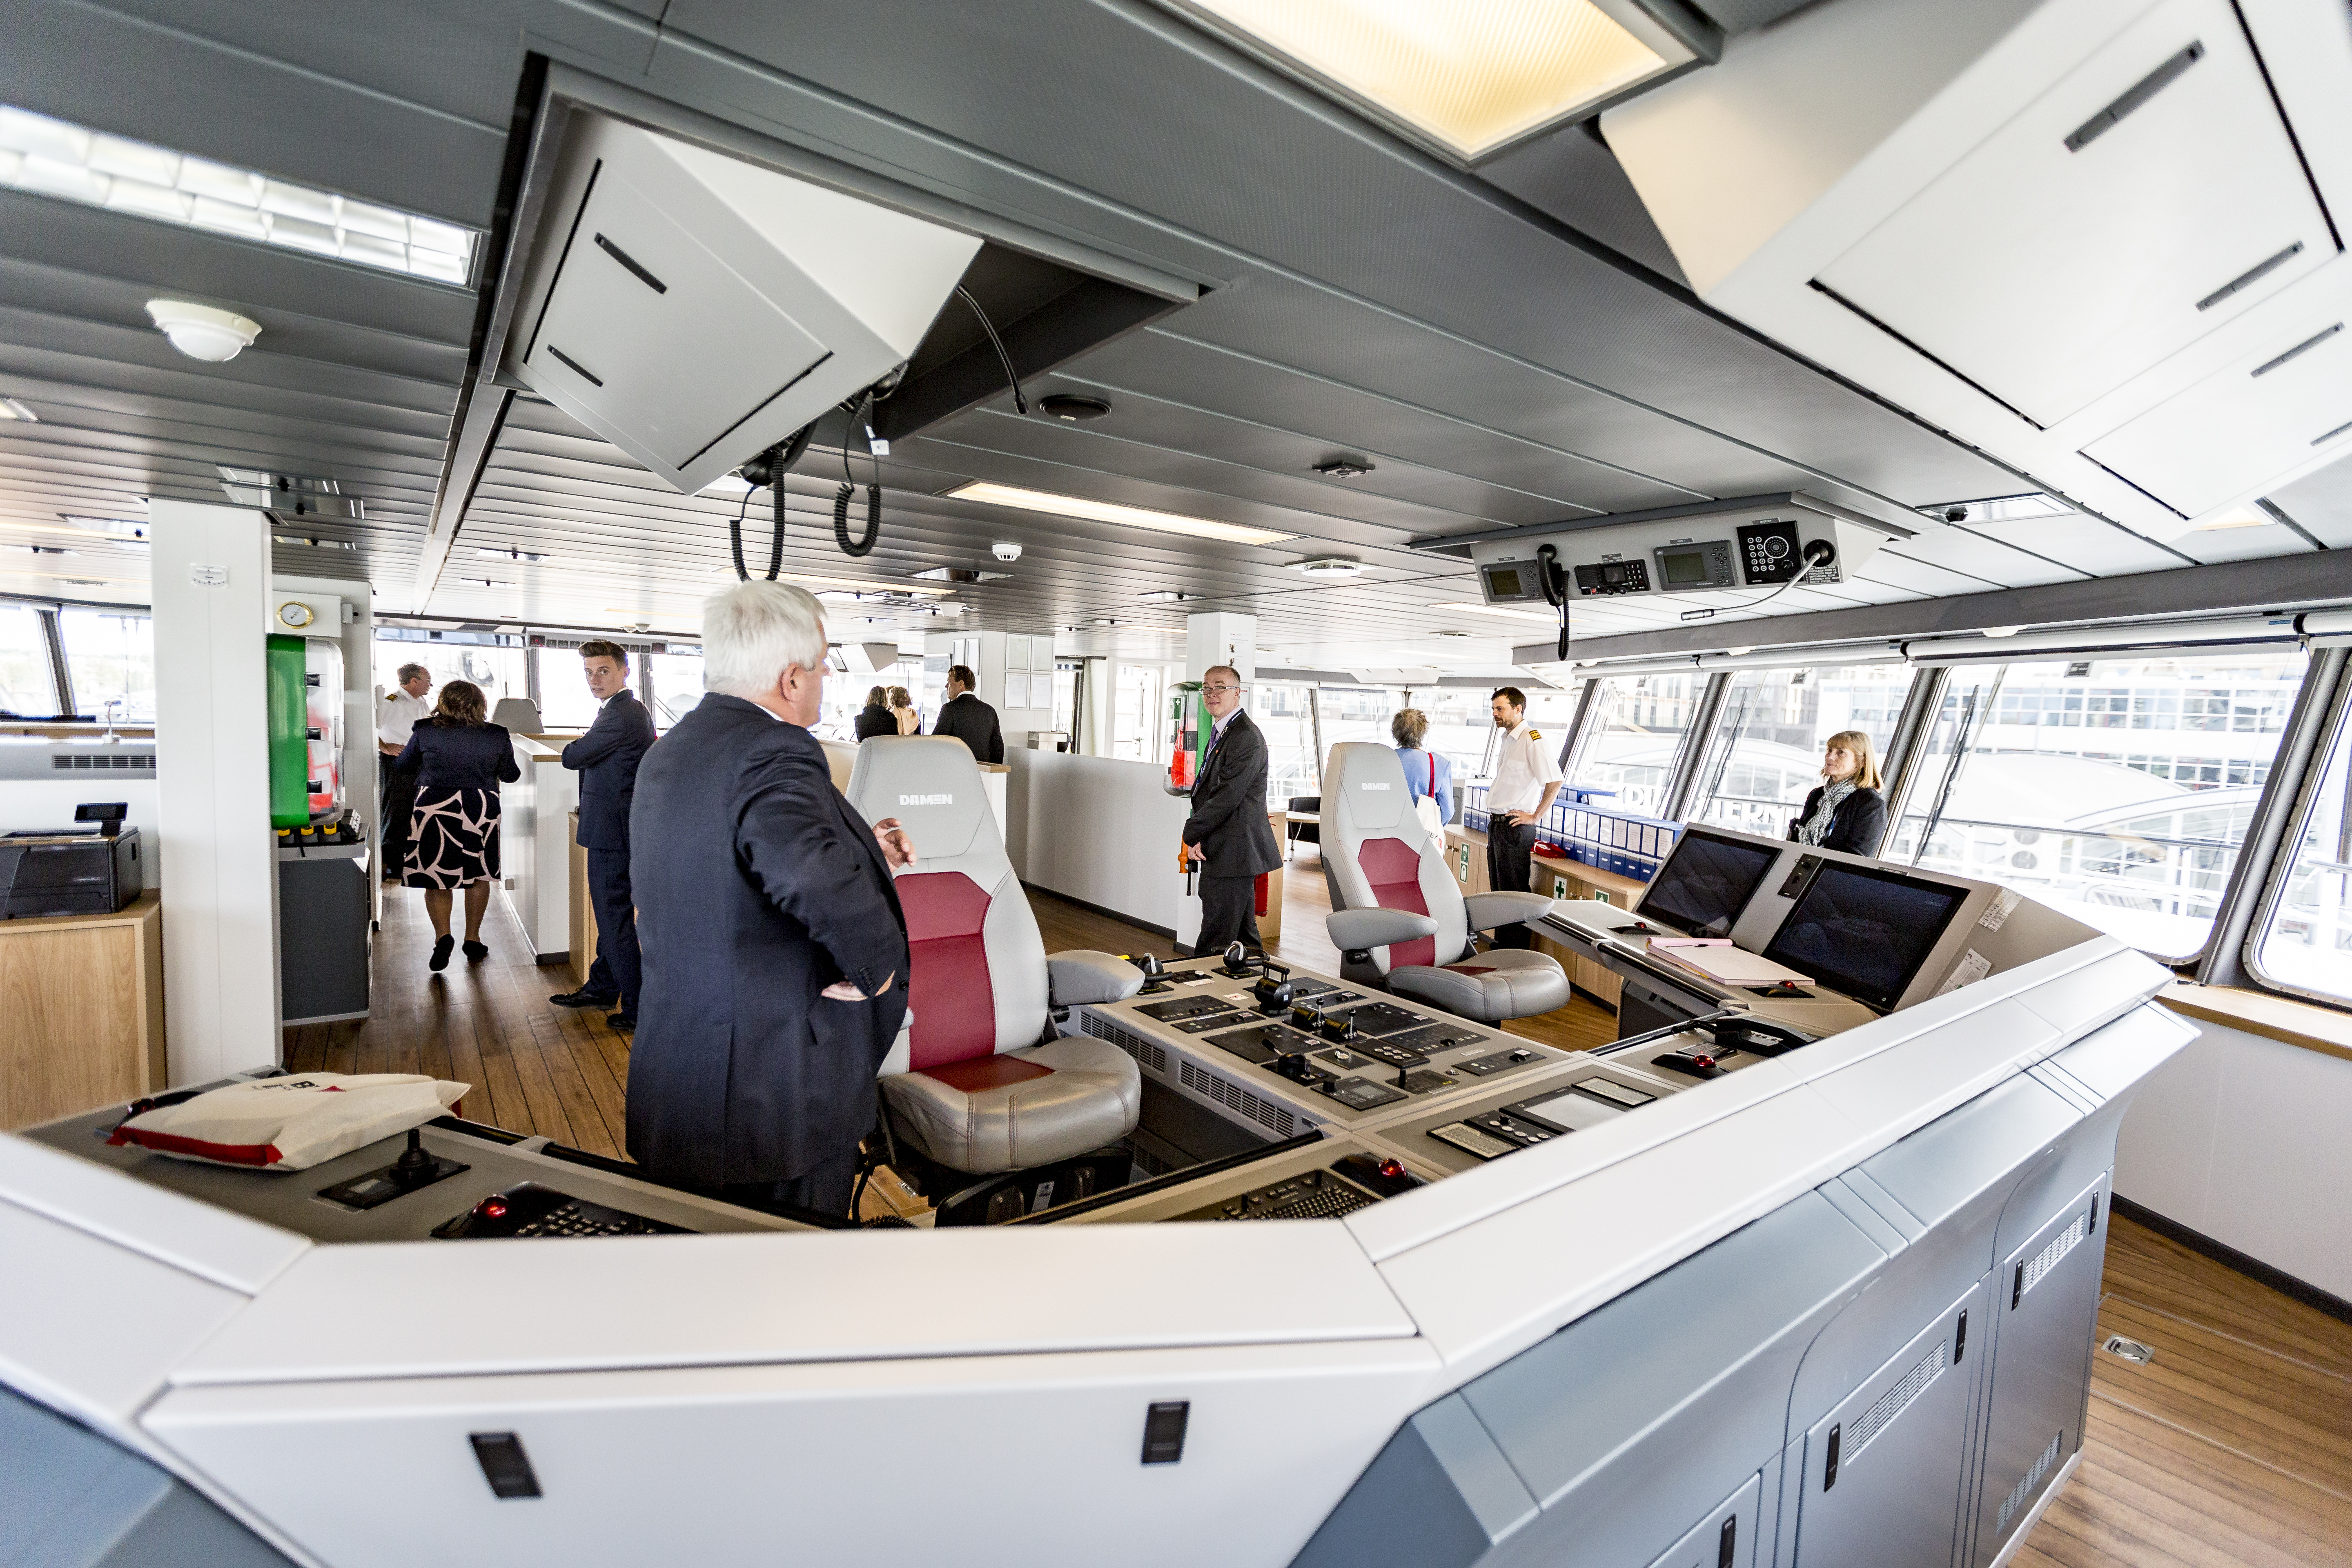
\includegraphics[width=\textwidth]{Brug-Bibby-Wavemaster.jpg}
		\caption{BIBBY WAVEMASTER 1}
	\end{subfigure}
	\hfill
	\begin{subfigure}[b]{0.45\textwidth}
		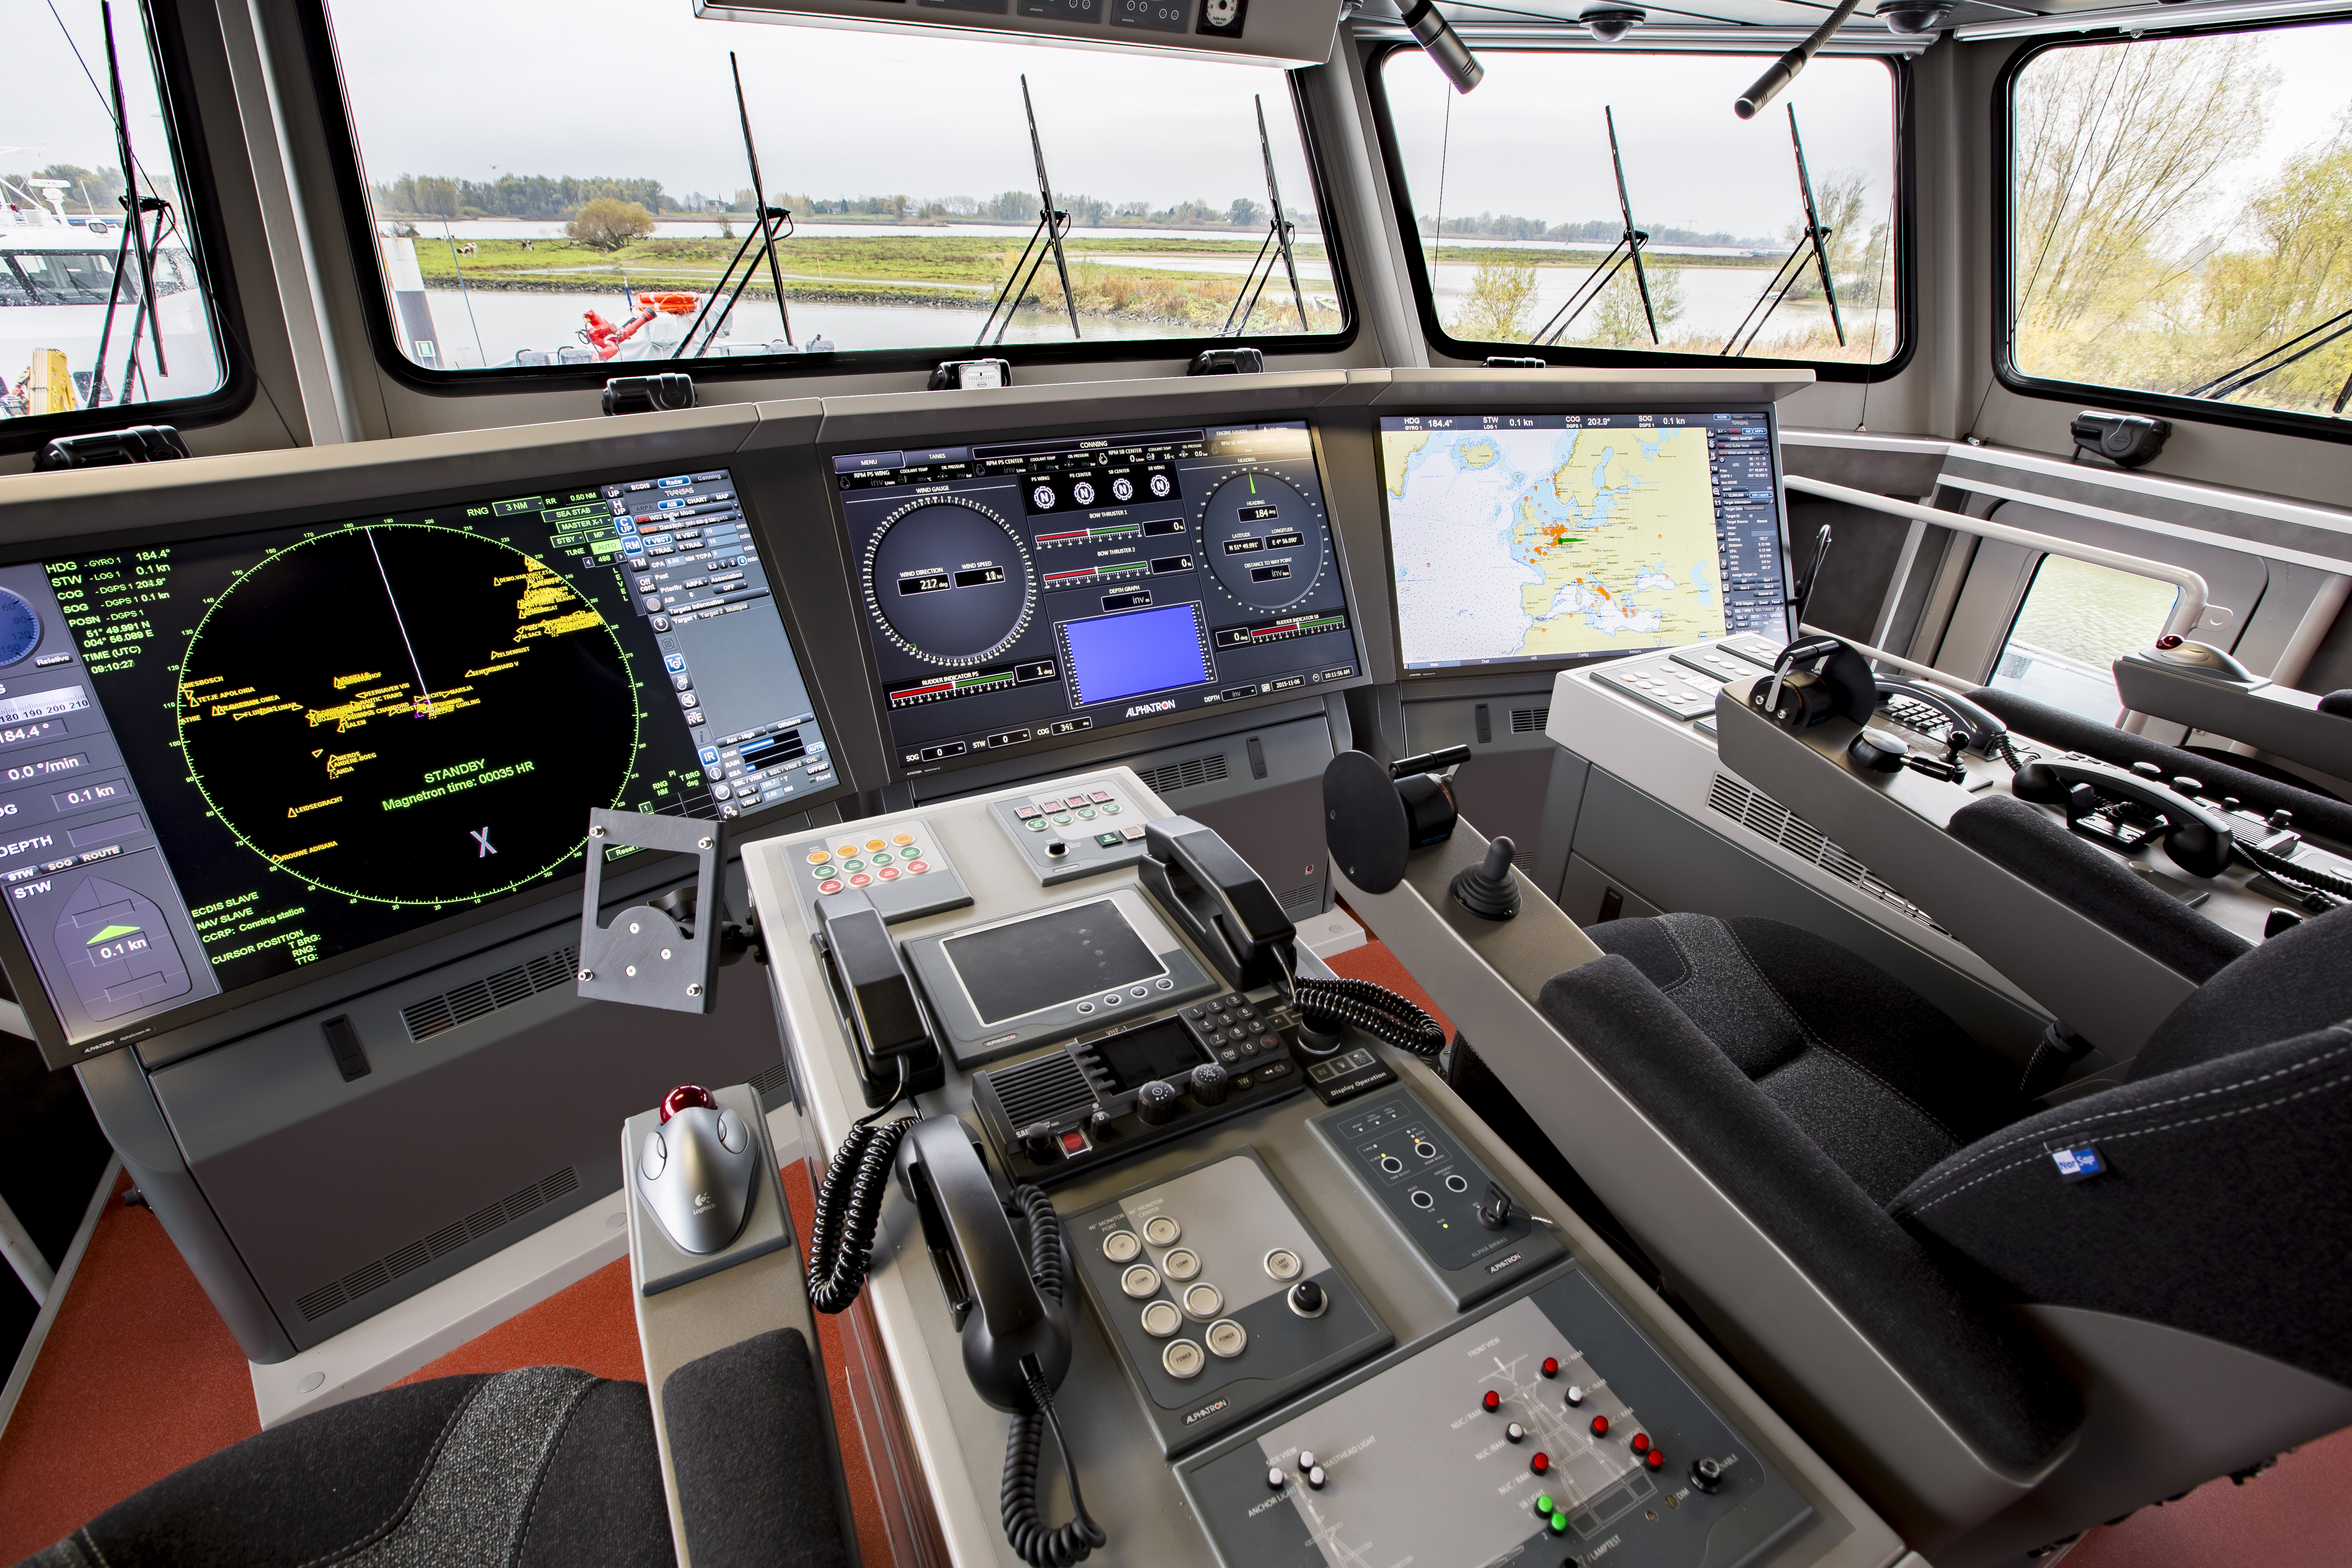
\includegraphics[width=\textwidth]{Brug-SPa-5009-Trinidad.jpg}
		\caption{DAMEN Stan Patrol 5009}
	\end{subfigure}	
	
	\caption{Various examples of bridge designs}
	\label{fig:bridge-example}
	
\end{figure}

\todo{How is information used. Mention parts on information overload. Thereby also the difference between ships. Officer walking around on big ship, vs small bridge on a tug for example.} 

\subsection{Human operator}
The human operator has two sides, to formal straight forward role as an operator. Which can be described with a list of tasks depending on their function. And the more difficult and unpredictable side of being a human. Which relates to the situational awareness and decision making ability.

\subsubsection{Role as operator}
\label{sec:deck-crew}
To give more insight into the different roles on board of a merchant's vessel, is the structure shown for officers in figure \ref{fig:crew-structure}. At smaller vessels, roles are combined where possible. The Navy has in some cases even more operational crew members. Apart from the licensed officers who manage the vessel, does the crew also consist of ratings who have hands-on skills within their own domain. \cite{Nedcon2013}

\tikzset{
	basic/.style   = {draw, text width=3cm, drop shadow, font=\sffamily, rectangle},
	root/.style    = {basic, thin, align=center, fill=gray!60},
	level 2/.style = {basic, thin, align=center, fill=gray!40},
	level 3/.style = {basic, thin, align=left, fill=gray!20, text width=8em, node distance = 25pt}
}
\begin{figure}[h]
	\centering
	\begin{tikzpicture}[
	level 1/.style={sibling distance=40mm},
	edge from parent/.style={->,draw},
	>=latex]
	
	% root of the the initial tree, level 1
	\node[root] {Master}
	% The first level, as children of the initial tree
	child {node[level 2] (c1) {Deck crew}}
	child {node[level 2] (c2) {Engine crew}};
	
	% The second level, relatively positioned nodes
	\begin{scope}[every node/.style={level 3}]
	\node [below of = c1, xshift=30pt] (c11) {Chief officer};
	\node [below of = c11] (c12) {Second officer};
	\node [below of = c12] (c13) {Third officer};
	\node [below of = c13] (c14) {Deck cadet};
	
	\node [below of = c2, xshift=30pt] (c21) {Chief engineer};
	\node [below of = c21] (c22) {First engineer};
	\node [below of = c22] (c23) {Second engineer};
	\node [below of = c23] (c24) {Third engineer};
	
	\end{scope}
	
	% lines from each level 1 node to every one of its "children"
	\foreach \value in {1,2,3,4}
	\draw[->] (c1.195) |- (c1\value.west);
	
	\foreach \value in {1,2,3,4}
	\draw[->] (c2.195) |- (c2\value.west);
	\end{tikzpicture}
	\caption{Basic crew structure organogram}
	\label{fig:crew-structure}
\end{figure}

For this research the Deck crew is most relevant, as they are in charge of the vessel navigation, watch keeping, maintaining the ship’s hull, cargo, gear and accommodation, taking care of the ship’s lifesaving and firefighting appliances. The deck department is also the one in charge of receiving, discharging and caring for cargo. According to the vessel’s hierarchy, the deck officers are as follows: Master, Chief Officer, Second Officer, Third Officer and Deck Cadet (deck officer to be).

The supreme authority on board a merchant's vessel is the Master or Captain. The entire crew is under his command. He is responsible for the safety, use and maintenance of the vessel and makes sure that every crew member carries out his work accordingly. He is also in charge of the following: payroll, ship’s accounting, inventories, custom and immigration regulations, and the ship’s documentation. In order to become Master, a seafarer must first have several years of experience as a deck officer and as Chief Officer.
According to the vessel’s hierarchy, the first deck officer and the head of the deck department after the Master is the Chief Officer. He is in charge of the vessel navigation, watch duties, charging and discharging operations. The Chief Officer also directs all the other officers on deck, creates and posts watch assignments and implements the Master’s orders in order to maintain safe operations and maintenance of the vessel.
Second Officer or Second Mate is the next in rank after the Chief Mate and is the ship’s navigator, focusing on creating the ship’s passage plans and keeping charts and publications up to date. Apart from watchkeeping, the Second Officer may also be designated to train the cadets on board or to fulfill the rank of security, safety, environmental or medical officer.
The Third Officer or Third Mate is the fourth deck officer in command and is usually the Ship’s Safety Officer, responsible for ensuring the good functioning of the fire-fighting equipment and lifesaving appliances. He undertakes bridge watches and learns how to become a Second Officer.
A Cadet on board a merchant's vessel receives structured training and experience on board and learns how to become a deck officer.

Apart from the officers, the deck department crew also consists of ratings, such as AB (Able Body Seaman), OS (Ordinary Seaman) and Boatswain.
The AB is part of the deck crew and has duties such as: taking watches, steering the vessel, assisting the Officer on watch, mooring and un-mooring the vessel, deck maintenance and cleaning. The AB also secures and un-secures the cargo and carries our deck and accommodation patrols.
OS is the crew member whose main duty is to maintain the cleanliness of the whole ship and serves as an assistant for the AB. Being an OS is considered to be an apprenticeship, a period called “sea time” in order to be allowed to take courses and training for AB.
Both AB and OS are usually supervised by a Boatswain, who is also a rating, in charge of examining the cargo-handling gear and lifesaving equipment as well. The Boatswain usually holds an AB certificate as well.
The structure for the deck department on board merchant vessels is mainly the same on all vessel types. \cite{Nedcon2013}

\subsubsection{Human factor}
At unmanned autonomous vessels the human operator will be replaced by a computer. This means that the duties as described above will be executed by a computer. This automation step has unknown consequences for the ability to observe and decision making. While it has clear advantages when it comes to memory and reduced concentration due to fatigue.

Situational awareness is a model to determine the ability to observe and make decisions. How well humans perform is determined by their (learning) experience \cite{Underwood2013}. Hereby is important to notice that situational awareness is not limited to perceiving, but has multiple levels. This is described using the Endsley model (figure \ref{fig:Endsley-SA-model}).

\begin{figure}[H]
	\centering
	\includegraphics[width=.8\textwidth]{Endsley-SA-model-png.png}
	\caption{Endsley model for situational awareness}
	\label{fig:Endsley-SA-model}
\end{figure}

The first step is to acquire situational awareness. This is based on three different levels of information processing \cite{Kalloniatis2017}: 
\begin{description}
	\item [Perception] Data is merely perceived.
	\item [Comprehension] Interpretation of data, enabling understanding of relevance in relation to tasks performed and goals to be attained. Forming a holistic picture of the operational environment. Identifying the significance of objects and events in that environment.
	\item [Projection] Making a forecast for likely future states of the situation. This is based on the interpreted data, experience and knowledge.
\end{description}

Based on the situational awareness, an decision is being made which results in an action. Changing the system and repeating the whole process. However there are factors which influence the effectiveness of this process. These can be internally or from the environment. Where automation is less prone to environmental factors, will it have a disadvantage when it comes to setting goals, preconceptions, acquiring knowledge or learning from experience. As many of the machine learning techniques are too much of a black box approach, or are not yet effective for the assignments where ships have to navigate for example. There’s also that indefinable matter of common sense that humans have but robots lack. Hundreds of thousands of years of evolution have provided us with a pretty good ability to recognize and make sense of things.

Whereas the human operator is more prone to environmental factors. Where workload is a big factor in the ability to concentrate and thus the ability to forecast future states and thus make the right decisions. The workload might be too high due to an overload of information \cite{Speier1999}, when tasks are too easy \cite{Washburn2001}, or when limited attention is desired for a long time, and something unexpected happens \cite{McMorris2018}.

These factors do only consider the single individual within the human operator team. But with larger ships there are multiple persons at the bridge, all with their own responsibilities. Research has shown that many of these crews have multiple cultures and nationalities work next to each other. Which often have a agreed working language which is not their first. This leads not only to minor irritations. But in some cases to hazardous situations \cite{Hetherington2006}. Certainly when conversations happen via a radio with some noise. 

\subsection{Procedures}
\label{apps:procedures}
To become a certified seafarer, different skills and knowledge must be acquired. The \ac{IMO} has developed several conventions to standardize this knowledge globally, the \ac{STCW} is leading here. This ensures that ships sailing in international waters have skilled crew which know what they can expect from other vessels. This also means they have navigational abilities such as plotting on a radar. But they also have knowledge of the conventions and systems used for safe navigation. Below some of these are explained in more detail. Followed by a description of known flaws of these systems and differences when compared to procedures used in practice.

\subsubsection{\acf{COLREGs}}
The \ac{COLREGs} set out the navigational to be followed by ships and other vessels at sea, to prevent collisions between two or more vessels. Although rules for navigating vessels inland may differ, the international rules specify that they should be as closely in line with the international rules as possible. In most of continental Europe, the Code Européen des Voies de la Navigation Intérieure (CEVNI, or the European Code for Navigation on Inland Waters) apply. In the United States, the rules for vessels navigating inland are published alongside the international rules.

Prior to the development of a single set of international rules and practices, there existed separate practices and various conventions and informal procedures in different parts of the world, as advanced by various maritime nations. As a result, there were inconsistencies and even contradictions that gave rise to unintended collisions. Vessel navigation lights for operating in darkness as well as navigation marks also were not standardised, giving rise to dangerous confusion and ambiguity between vessels at risk of colliding. Different nations already came up with their own set of rules. But the first version was amended together with \ac{SOLAS} in 1960. Additions were made including traffic separation schemes in 1972.

The \ac{COLREGs} includes 41 rules divided into six sections: Part A - General; Part B - Steering and Sailing; Part C - Lights and Shapes; Part D - Sound and Light signals;  Part E - Exemptions; and Part F - Verification of compliance with the provisions of the Convention. There are also four Annexes containing technical requirements concerning lights and shapes and their positioning; sound signalling appliances; additional signals for fishing vessels when operating in close proximity, and international distress signals.

Where part B is most relevant for this research, with subject like safe speed, obligation to determine risk of collision and take action with all means available, how to act in different situations with other ships, or in restricted waterways. 

\subsubsection{\acf{SMCP}}
As navigational and safety communications from ship to shore and vice versa, ship to ship , and on board ships must be precise, simple and unambiguous, so as to avoid confusion and error, there is a need to standardize the language used. This is of particular importance in the light of the increasing number of internationally trading vessels with crews speaking many different languages since problems of communication may cause misunderstandings leading to dangers to the vessel, the people on board and the environment.

In 1973 \ac{IMO} started to develop the \acf{SMNV}, which was replaced by the \ac{SMCP} in 2001. The ability to understand and use the \ac{SMCP} is required for the certification of officers in charge of a navigational watch on ships of 500 gross tonnage or more. To assist in greater safety of navigation and of the conduct of the ship. To standardize the language used in communication for navigation at sea, in port-apporaches, in waterways, harbours and on board vessels with multilingual crews. Which is all instructed at maritime training institutions. These are not intended to supplant or contradict \ac{COLREGs} or special local rules or recommendations made by IMO concerning ship routeing. Just as radiotelephone procedures should be followed strictly as set out in the ITU Radio Regulations. 

It is a collection of phrases used to standardize and simplify the communication, where synonyms and contracted forms are avoided. Some \href{http://www.segeln.co.at/media/pdf/smcp.pdf}{examples of the usage of \ac{SMCP}} are shown below, including message markers to indicate the type of message:
\begin{description}
	\item [Advice] Stand by on channel 6 - 8.
	\item [Information] The fairway entrance is: position: bearing 1-3-7 degrees true from North Point Lighthouse, distance: 2 decimal 3 miles.
	\item [Warning] Buoy number: one - five unlit.
	\item [Intention] I intend to reduce speed, new speed: eight knots.
	\item [Question] What are your intentions?
	\item [Instruction] You must alter course to starboard.
	\item [Request] Immediate tug assistance.
\end{description}

\section{Difference between theory and practice}

\todo{How does it go in practice, experience.}

Certainly in inland water or near coast conversations might be in natural language, instead of \ac{SMCP}.

Mention the problems with ECDIS/AIS (old information, not correct as mentioned by loodswezen), as I refer to this in snapshots scenario description. 

\section{Relevant systems for autonomous shipping}
\label{sec:relevant-systems}
Not everything is relevant to other ships, in order to determine the possible decisions. This is only: information from radar, information available in AIS (where reliability must be considered), warning systems, etc...

\todo{Write into a story}

\begin{itemize}
	\item Radio communication
	\begin{itemize}
		\item Conversational agent using \acf{SMCP}
		\item Availability on \acf{VHF}
		\item \acf{AIS} messages
	\end{itemize}
	\item Visible signals
	\begin{itemize}
		\item Light signals
		\item Flags
		\item Mast head signals
		\item Heading, position and movements
	\end{itemize}
	\item Audible signals
	\begin{itemize}
		\item Horn
		\item Speakers
	\end{itemize}
	\item Distress, urgency and safety signals
	\begin{itemize}
		\item Flares
		\item Smoke
	\end{itemize}
\end{itemize}

e.g: VDES